\documentclass{article}
\usepackage{physics}
\usepackage{graphicx}
\usepackage{caption}
\usepackage{amsmath}
\usepackage{bm}
\usepackage{framed}
\usepackage{authblk}
\usepackage{empheq}
\usepackage{amsfonts}
\usepackage{esint}
\usepackage[makeroom]{cancel}
\usepackage{dsfont}
\usepackage{centernot}
\usepackage{mathtools}
\usepackage{subcaption}
\usepackage{bigints}
\usepackage{amsthm}
\theoremstyle{definition}
\newtheorem{lemma}{Lemma}
\newtheorem{defn}{Definition}[section]
\newtheorem{prop}{Proposition}[section]
\newtheorem{rmk}{Remark}[section]
\newtheorem{thm}{Theorem}[section]
\newtheorem{exmp}{Example}[section]
\newtheorem{prob}{Problem}[section]
\newtheorem{sln}{Solution}[section]
\newtheorem*{prob*}{Problem}
\newtheorem{exer}{Exercise}[section]
\newtheorem*{exer*}{Exercise}
\newtheorem*{sln*}{Solution}
\usepackage{empheq}
\usepackage{tensor}
\usepackage{xcolor}
%\definecolor{colby}{rgb}{0.0, 0.0, 0.5}
\definecolor{MIT}{RGB}{163, 31, 52}
\usepackage[pdftex]{hyperref}
%\hypersetup{colorlinks,urlcolor=colby}
\hypersetup{colorlinks,linkcolor={MIT},citecolor={MIT},urlcolor={MIT}}  
\usepackage[left=1in,right=1in,top=1in,bottom=1in]{geometry}
\setcounter{MaxMatrixCols}{20}
\usepackage{newpxtext,newpxmath}
\newcommand*\widefbox[1]{\fbox{\hspace{2em}#1\hspace{2em}}}

\newcommand{\p}{\partial}
\newcommand{\R}{\mathbb{R}}
\newcommand{\C}{\mathbb{C}}
\newcommand{\lag}{\mathcal{L}}
\newcommand{\nn}{\nonumber}
\newcommand{\ham}{\mathcal{H}}
\newcommand{\M}{\mathcal{M}}
\newcommand{\I}{\mathcal{I}}
\newcommand{\K}{\mathcal{K}}
\newcommand{\F}{\mathcal{F}}
\newcommand{\w}{\omega}
\newcommand{\lam}{\lambda}
\newcommand{\al}{\alpha}
\newcommand{\be}{\beta}
\newcommand{\x}{\xi}

\newcommand{\G}{\mathcal{G}}

\newcommand{\f}[2]{\frac{#1}{#2}}

\newcommand{\ift}{\infty}

\newcommand{\lp}{\left(}
\newcommand{\rp}{\right)}

\newcommand{\lb}{\left[}
\newcommand{\rb}{\right]}

\newcommand{\lc}{\left\{}
\newcommand{\rc}{\right\}}


\newcommand{\V}{\mathbf{V}}
\newcommand{\U}{\mathcal{U}}
\newcommand{\Id}{\mathcal{I}}
\newcommand{\D}{\mathcal{D}}
\newcommand{\Z}{\mathcal{Z}}

%\setcounter{chapter}{-1}


\usepackage{enumitem}



\usepackage{listings}
\captionsetup[lstlisting]{margin=0cm,format=hang,font=small,format=plain,labelfont={bf,up},textfont={it}}
\renewcommand*{\lstlistingname}{Code \textcolor{violet}{\textsl{Mathematica}}}
\definecolor{gris245}{RGB}{245,245,245}
\definecolor{olive}{RGB}{50,140,50}
\definecolor{brun}{RGB}{175,100,80}

%\hypersetup{colorlinks,urlcolor=colby}
\lstset{
	tabsize=4,
	frame=single,
	language=mathematica,
	basicstyle=\scriptsize\ttfamily,
	keywordstyle=\color{black},
	backgroundcolor=\color{gris245},
	commentstyle=\color{gray},
	showstringspaces=false,
	emph={
		r1,
		r2,
		epsilon,epsilon_,
		Newton,Newton_
	},emphstyle={\color{olive}},
	emph={[2]
		L,
		CouleurCourbe,
		PotentielEffectif,
		IdCourbe,
		Courbe
	},emphstyle={[2]\color{blue}},
	emph={[3]r,r_,n,n_},emphstyle={[3]\color{magenta}}
}

\newcommand{\diag}{\text{diag}}
\newcommand{\psirot}{\ket{\psi_\text{rot}(t)} }
\newcommand{\RWA}{\ham_\text{rot}^\text{RWA}}

% 3j symbol
\newcommand{\tj}[6]{ \begin{pmatrix}
		#1 & #2 & #3 \\
		#4 & #5 & #6 
\end{pmatrix}}


\begin{document}
\begin{framed}
\noindent Name: \textbf{Huan Q. Bui}\\
Course: \textbf{8.421 - AMO I}\\
Problem set: \textbf{\#10}\\
Due: Friday, April 22, 2022.
\end{framed}



\noindent \textbf{1. Optical Bloch Equation with Spontaneous Emission. } Here we have a two level system $\{ \ket{a}, \ket{b} \}$ driven with Rabi frequency $\omega_R$ with damping rate $\Gamma$. We will compute the population fraction in the excited state $\ket{b}$ as $t\to \infty$. 

\begin{enumerate}[label=(\alph*)]
	\item We will begin by guessing the population in the excited state $\ket{b}$ in the limit $t\to \infty$ in the large detuning $|\delta| \ll \omega_R, \Gamma$ limit. 
	\begin{enumerate}[label=(\roman*)]
		\item $\rho_{bb}(t)$ from undamped Rabi oscillation is given by 
		\begin{align*}
		\rho_{bb}(t) = \f{\omega_R^2}{\omega_R^2 + \delta^2} \sin^2\lp \f{\sqrt{\omega_R^2 + \delta^2}}{2} t \rp.
		\end{align*}
		Suppose there is a weak damping term present. Assume further that the oscillatory term will damp out to the average value, then we expect an additional $\Gamma^2$ term in the denominator of the leading factor and that the $\sin^2$ term averages to $1/2$, so
		\begin{align*}
		\rho_{bb}(t) \to \f{\omega_R^2/2}{\omega_R^2 + \delta^2 + \Gamma^2}.
		\end{align*}
		Note that the initial condition leading to the initial solution doesn't matter when we consider the large time and large detuning limits.
		
		
		\item In the setup where we have two state $\ket{a,1}$ and $\ket{b,0}$ coupled by $\ham_\text{int} = -\bm{d}\cdot \bm{E} $ with $\bm{E} = i\sqrt{2\pi \hbar \omega/V} (a - a^\dagger)$. Since the driving field is off-resonant, we can't use the treatment given in Section 7.6 of the lecture notes. However, we're already very close. Let the system be in the state
		\begin{align*}
		\ket{\psi(t)} =  c_{a,0}(t) \ket{a,0} + c_{b,1}(t)\ket{b,1}.
		\end{align*}
		The Hamiltonian which generates the time evolution of the system is given by 
		\begin{align*}
		\ham = \ham_A + \ham_\text{int} + \hbar \omega a^\dagger a
		\end{align*}
		where $\ham_A$ represents the atom Hamiltonian. Applying the Schr\"{o}dinger equation, we find the following system of differential equations:
		\begin{align*}
		&\p_t c_{a,0}(t) = -i\omega_0 c_{a,0}(t) - \f{i\omega_R}{2} c_{b,1}(t)\\
		&\p_t c_{b,1}(t) = -i\omega c_{b,1}(t) - \f{i\omega_R}{2} c_{a,0}(t).
		\end{align*}
		It turns out that this is nothing more than the Rabi problem which we have done before. The excited state population fraction is given by 
		\begin{align*}
		\rho_{bb}(t) = \f{\omega_R^2}{\omega_R^2 + \delta^2} \sin^2 \lp  \f{\sqrt{\omega_R^2 + \delta^2}}{2}  t \rp.
		\end{align*}
		So, in the large time and large detuning limit with small damping as considered above, we may make (the same) guess:
		\begin{align*}
		\rho_{bb}(t) \to \f{\omega_R^2/2}{\omega_R^2 + \delta^2 + \Gamma^2}.
		\end{align*}
	\end{enumerate}
	
	\item Here we properly consider the effect of spontaneous emission. To this end, we consider the time evolution of the density matrix 
	\begin{align*}
	\rho = \begin{pmatrix}
	\rho_{aa} & \rho_{ab} \\ \rho_{ba} & \rho_{bb}
 	\end{pmatrix}.
	\end{align*}
	Denote the damping rate for the populations as $\Gamma_1$ and the damping rate for the coherences as $\Gamma_2$. The evolution of the system, including spontaneous emission, can be completely determined by the following equation of motion (the \textbf{optical Bloch equation(s)}):
	\begin{align*}
	\dot\rho = \f{1}{i\hbar}[\ham, \rho] + \begin{pmatrix}
	\Gamma_1 \rho_{bb} & -\Gamma_2 \rho_{ab} \\ -\Gamma_2 \rho_{ba} & -\Gamma_1 \rho_{bb}
	\end{pmatrix}
	\end{align*}
	where 
	\begin{align*}
	\ham = \f{\hbar}{2}\begin{pmatrix}
	-\omega_0 & \omega_r e^{i\omega t} \\ \omega_R e^{-i \omega t} & \omega_0
	\end{pmatrix}
	\end{align*}
	and $\rho_{aa} + \rho_{bb} =1$, $\rho_{ab} = \rho^*_{ba}$. We are interested only in the steady state solution, so we won't solve this system explicitly. 
	
	\begin{enumerate}[label=(\roman*)]
		\item Consider the substitutions:
		\begin{align*}
		&\hat{\rho}_{ab} = \rho_{ab} e^{-i\omega t} \\ 
		&\hat{\rho}_{ba} = \rho_{ba} e^{i\omega t}.
		\end{align*}
		The system of equations above becomes
		\begin{align*}
		\dot{\rho}_{aa} &= \f{1}{i\hbar}\lp -\f{\hbar}{2} \rho_{ab} \omega_R e^{-i\omega t} + \f{\hbar}{2} \rho_{ba}\omega_R e^{i\omega t } \rp + \Gamma_1 \rho_{bb}\\
		& = \f{+i\omega_R}{2} \lp \hat{\rho}_{ab} - \hat{\rho}_{ba} \rp + \Gamma_1 \rho_{bb}\\
		\dot{\rho}_{bb} &= \f{1}{i\hbar}\lp +\f{\hbar}{2} \rho_{ab} \omega_R e^{-i\omega t} - \f{\hbar}{2}\rho_{ba} \omega_R e^{i\omega t} \rp -\Gamma_1 \rho_{bb}\\
		& = \f{-i\omega_R}{2}\lp \hat{\rho}_{ab} - \hat{\rho}_{ba} \rp - \Gamma_1 \rho_{bb}\\
		\dot{\hat{\rho}}_{ab} &= \dot{\rho}_{ab}e^{-i\omega t} - i\omega \rho_{ab} e^{-i\omega t}\\
		& =  -ie^{-i\omega t}\lp - \rho_{ab} \omega_0 - \f{\omega_R}{2}\rho_{aa} e^{i\omega t} + \f{\omega_R}{2} \rho_{bb}  e^{i\omega t}  \rp -\Gamma_2 \rho_{ab}e^{-i\omega t} - i\omega \rho_{ab}e^{-i\omega t}\\
		&= (-i\delta - \Gamma_2)\hat{\rho}_{ab} + \f{i\omega_R}{2}(\rho_{aa} - \rho_{bb})\\
		\dot{\hat{\rho}}_{ba} &= \dot{\rho}_{ba} e^{i\omega t} + i\omega \rho_{ba} e^{i\omega t} \\
		&= -ie^{i\omega t}\lp \rho_{ba} \omega_0 + \f{\omega_R}{2}\rho_{aa} e^{-i\omega t} - \f{\omega_R}{2} \rho_{bb}  e^{-i\omega t}  \rp - \Gamma_2 \rho_{ba}e^{i\omega t} + i\omega \rho_{ba}e^{i\omega t}\\
		&= (+i\delta - \Gamma_2 ) \hat{\rho}_{ba} - \f{i\omega_R }{2} (\rho_{aa} - \rho_{bb})
		\end{align*}
		where $\delta = \omega - \omega_0$.
		
		
		
		
		
		\item We now wish to solve for $\rho_{bb}$ in steady state, $t\to \infty$. To this end, we set all time derivatives above to zero and obtain the following system:
		\begin{align*}
		0 & = \f{+i\omega_R}{2} \lp \hat{\rho}_{ab} - \hat{\rho}_{ba} \rp + \Gamma_1 \rho_{bb}\\
		0 & = \f{-i\omega_R}{2}\lp \hat{\rho}_{ab} - \hat{\rho}_{ba} \rp - \Gamma_1 \rho_{bb}\\
		0 &= (-i\delta - \Gamma_2)\hat{\rho}_{ab} + \f{i\omega_R}{2}(\rho_{aa} - \rho_{bb})\\
		0
		&= (+i\delta - \Gamma_2 ) \hat{\rho}_{ba} - \f{i\omega_R }{2} (\rho_{aa} - \rho_{bb}).
		\end{align*}
		The first two equations are actually just one. From the last two equations we find 
		\begin{align*}
		\Gamma_1 \rho_{bb} 
		&= -\f{i\omega_R}{2}(\hat{\rho}_{ab} - \hat{\rho}_{ba}) \\
		&= -\f{i\omega_R}{2} \f{i\omega_R}{2}(\rho_{aa} - \rho_{bb})\f{(-i\delta - \Gamma_2) - (i\delta - \Gamma_2)}{\delta^2 + \Gamma_2^2} \\
		&= \f{\omega_R^2}{2}(1-2\rho_{bb}) \f{\Gamma_2}{\delta^2 + \Gamma_2^2}.
		\end{align*}
		From here, we find 
		\begin{align*}
		\rho_{bb} = \f{\omega_R^2}{2}\f{\Gamma_2/\Gamma_1}{\delta^2 + \Gamma_2^2 + \f{\Gamma_2}{\Gamma_1}\omega_R^2},
		\end{align*}
		as desired. 
	\end{enumerate}
	
	\item Now we need to represent $\Gamma_1$ and $\Gamma_2$ in terms of the spontaneous emission rate $\Gamma$. 
	\begin{enumerate}[label=(\roman*)]
		\item When there is no driving force, $\ham = 0$, the density matrix $\rho$ evolves as
		\begin{align*}
		\dot\rho
		= \begin{pmatrix}
		\dot{\rho}_{aa} & \dot{\rho}_{ab} \\ \dot{\rho}_{ba} & \dot{\rho}_{bb}
		\end{pmatrix} 
		= \begin{pmatrix}
		\Gamma_1 \rho_{bb} & -\Gamma_2 \rho_{ab} \\ -\Gamma_2 \rho_{ba} & -\Gamma_1 \rho_{bb}
		\end{pmatrix}
		\end{align*}
		By inspection, we can readily solve for $\rho(t)$:
		\begin{align*}
		\rho(t) = \begin{pmatrix}
		1 - [1- \rho_{aa}(0)]e^{-\Gamma_1 t} & \rho_{ab}(0) e^{-\Gamma_2 t} \\ 
		\rho_{ba}(0)e^{-\Gamma_2 t} &  \rho_{bb}(0) e^{-\Gamma_1 t}
		\end{pmatrix} = \begin{pmatrix}
		1 - \rho_{bb}(0)e^{-\Gamma_1 t} & \rho_{ab}(0) e^{-\Gamma_2 t} \\ 
		\rho_{ba}(0)e^{-\Gamma_2 t} &  \rho_{bb}(0) e^{-\Gamma_1 t}
		\end{pmatrix}
		\end{align*}
		
		\item Suppose that the atom starts out in a superposition state
		\begin{align*}
		\ket{\psi(0)} = (\al_a (0) \ket{a } + \al_b (0) \ket{b})
		\otimes \ket{0},
		\end{align*}
		then at time $t$ it will be in the state
		\begin{align*}
		\ket{\psi(t)} =  \al_a(t) \ket{a} \otimes \ket{0} + \al_b(t) \ket{b} \otimes \ket{0} + \sum_k c_k(t) \ket{a} \otimes \ket{1_k}
		\end{align*}
		where $\ket{n_k}$ is an $n$-photon state in mode $k$. The density matrix for the atom, $\rho$ is the reduced density matrix of the atom + photon system given by $\ket{\psi(t)} \bra{\psi(t)}$. Specifically, $\rho$ is $\ket{\psi(t)} \bra{\psi(t)}$, with the photon part traced out:
		\begin{align*}
		\rho(t) &= \Tr_\text{F}\ket{\psi(t)} \bra{\psi(t)} \\
		&= 
		|\al_a(t)|^2 \ket{a}\bra{a}  \Tr_\text{F}(\ket{0}\bra{0})
		+ 
		|\al_b(t)|^2 \ket{b}\bra{b}  \Tr_\text{F}(\ket{0}\bra{0}) 
		+ 
		\sum_{k,j} c_k(t)c_j^*(t) \ket{a}\bra{a}  \Tr_\text{F}(\ket{1_k}\langle{1_j}|)\\
		&\quad +
		\al_a(t)\al_b^*(t) \ket{a}\bra{b}  \Tr_\text{F}(\ket{0}\bra{0}) 
		+ 
		\al_b(t)\al_a^*(t) \ket{b}\bra{a}  \Tr_\text{F}(\ket{0}\bra{0}) \\
		&\quad + 
		\cancel{\sum_k c_k(t) \al_a^*(t) \ket{a}\bra{a}  \Tr_\text{F}(\ket{1_k}\bra{0})} + 
		\cancel{\sum_j c_j^*(t)\al_a(t) \ket{a}\bra{a}  \Tr_\text{F}(\ket{0}\bra{1_j}) }\\
		&\quad + 
		\cancel{\sum_k c_k(t)\al_b^*(t) \ket{a}\bra{b}  \Tr_\text{F}(\ket{1_k}\bra{0})} + 
		\cancel{\sum_j c_j^*(t) b(t) \ket{b} \bra{a}  \Tr_\text{F}(\ket{0}\bra{1_j})}\\
		&= |\al_a(t)|^2 \ket{a}\bra{a} + |\al_b(t)|^2 \ket{b}\bra{b} + \al_a(t)\al_b^*(t) \ket{a}\bra{b} 
		+ 	\al_b(t)\al_a^*(t) \ket{b}\bra{a} + \sum_k |c_k(t)|^2 \ket{a}\bra{a}\\
		&= \begin{pmatrix}
		|\al_a(t)|^2+ \sum_k |c_k(t)|^2 & \al_a(t)\al_b^*(t) \\ 
		\al_a^*(t)\al_b(t)  & |\al_b(t)|^2  
		\end{pmatrix}
		\end{align*}
		Here, "$\text{F}$" denotes the Fock space which contains the photon number states. By comparing this result to that in Part (i), we can first identify 
		\begin{align*}
		|\al_b(t)|^2 \sim e^{-\Gamma_1 t}. 
		\end{align*}
		Since the population in the excited state, $\rho_{bb}$ decays like $e^{-\Gamma t}$, we must have that
		\begin{align*}
		\Gamma_1 = \Gamma.
		\end{align*}
		Due to spontaneous decay, the decrease in the amplitude $\al_b(t)$ contributes to the increase in the amplitude $c_k(t)$. As a result, we may argue that the amplitude of the eigenstate $\ket{a} \otimes \ket{0}$ does not decay exponentially, i.e.  
		\begin{align*}
		e^{-\Gamma_2 t} \sim \al_a^*(t) \al_b(t)  \sim e^{-\Gamma_1 t/2}  = e^{-\Gamma t /2},
		\end{align*}
		from which we conclude that 
		\begin{align*}
		\Gamma_2 = \f{\Gamma}{2},
		\end{align*}
		as desired. To explain \textit{why} the off-diagonal elements decay at half rate of the excited population, we can make an analogy between the two-level system and a damped undriven harmonic oscillator. The energy of the two-level system is proportional the excited state population $E \propto \rho_{22}$. Now consider the damped undriven harmonic oscillator given by 
		\begin{align*}
		\ddot{x} + \be \dot{x} + \omega_0^2 x = 0
		\end{align*}
		whose (steady-state) solution is given by 
		\begin{align*}
		x(t) = U(t)\cos \omega t - V(t)\sin\omega t.
		\end{align*} 
		Here, the "amplitudes" $U(t), V(t)$ satisfy:
		\begin{align*}
		&\dot{U} = -\omega_0 V- \f{\be}{2} U \\ 
		&\dot{V} = \omega_0 U - \f{\be}{2}V
		\end{align*}
		and the time-evolution of the total energy is simply
		\begin{align*}
		\dot E = -\be E.
		\end{align*}
		By identifying $\rho_{bb}$ with $E$, we see that $\Gamma$ plays the role of $\be$. By identifying $U$ with the coherences, aka the off-diagonal terms in the density matrix, we see that they decay exponentially with rate $\Gamma/2$ as found before. Alternatively, one can see all of this by realizing that $E\propto x^2$, implying if $E\sim e^{-\Gamma t}$ then $x\sim e^{-\Gamma t/2 }$.
	\end{enumerate}
	

	
	\item It turns out that the relations $\Gamma_1 = \Gamma = 2\Gamma_2 $ still hold in the presence of the driving force. 
	
	
	\begin{enumerate}[label=(\roman*)]
		\item With this, we can rewrite the steady-state solution for $\rho_{bb}$ as follows:
		\begin{align*}
		\rho_{bb} &= \f{\omega_R^2}{2}\f{\Gamma_2/\Gamma_1}{\delta^2 + \Gamma_2^2 + \f{\Gamma_2}{\Gamma_1}\omega_R^2}\\
		&= \f{\omega_R^2}{4}\f{1}{\delta^2 + \Gamma^2/4 + \omega_R^2/2}\\
		&= \f{\omega_R^2}{\Gamma^2}\f{1}{1 + 4\delta^2/\Gamma^2 + 2\omega_R^2/\Gamma^2}\\
		&= \f{s/2}{1+4\delta^2/\Gamma^2 + s}.
		\end{align*}
		
		
		
		\item In the large detuning limit, $\abs{\delta} \gg \Gamma, \omega_R$, we have
		\begin{align*}
		\rho_{bb} \approx \f{s/2}{4\delta^2/\Gamma^2} = \f{\omega_R^2}{4\delta^2},
		\end{align*}
		which is off from our guess in part (a) by a factor of 2, which comes from the ratio between the spontaneous decay rate and the dephasing rate $\Gamma_1/\Gamma_2 = 2$. 
	\end{enumerate}
\end{enumerate}


\noindent \textbf{2. Intensity Distribution Due to Spontaneous Emission. } Here we consider an atom of total angular momentum $J$ with spontaneous emission rate $A$. It radiates to a lower level with angular momentum $J' = J-1$.We want to find the rates for the various allowed transitions, i.e. the fraction of the radiation that goes into each of the possible transitions $(J,m) \to (J',m')$. The rates can be found by applying the following rules:
\begin{itemize}
	\item The sum of the rates of of each state $(J,m)$ must equal $A$.
	\item The sum of the rates into each state $(J',m')$ must equal $A(2J+1)/(2J'+1)$.
	\item An unpolarized mixture of radiators in level $J$ must emit equal intensities of light with each of the three polarization components.
	\item The rate for a transition $(J,m)\to (J',m')$ must be the same as for $(J,-m)\to (J',m')$.
\end{itemize}
For $J=2,J'1=2$, designate the transitions by letters as follows:
\begin{align*}
&a:\quad m=2 \to m'=1\\
&b:\quad m=1 \to m'=1\\
&c:\quad m=0 \to m'=1\\
&d:\quad m=1\to m'=0\\
&e:\quad m=0 \to m'=0
\end{align*}

\begin{enumerate}[label=(\alph*)]
	\item Here we find the rates for $a$ through $e$ using the rules above. The third rule says that the sum of the rates for the three possible $\Delta m$'s are the same. We have the following system of five equations with five unknowns:
	\begin{align*}
	&\Gamma_a = A \\
	&\Gamma_b+ \Gamma_d = A \\
	& 2\Gamma_c + \Gamma_e = A\\
	&\Gamma_a + \Gamma_b + \Gamma_c = A \f{2\times 2+1}{2\times 1 + 1} = \f{5A}{3}\\
	& \Gamma_a + \Gamma_d + \Gamma_c = 2\Gamma_b + \Gamma_e
	\end{align*} 
	Solving this system gives
	\begin{align*}
	\Gamma_a = A, \quad \Gamma_b = \f{A}{2}, \quad \Gamma_c = \f{A}{6}, \quad \Gamma_d = \f{A}{2}, \quad \Gamma_e = \f{2A}{3}.
	\end{align*}
	
	
		
	\item Here we find the rates for $a$ through $e$ using the Wigner-Eckart theorem, which states that
	\begin{align*}
	\bra{J m_J} T_{Lm} \ket{J'm_{J'}} = c(J'LJ; m_{J'}mm_J) \langle J \norm{T_L} J'\rangle \propto \bra{J'm_{J'}}\ket{k,q; J,m_J} 
	\end{align*} 
	where $k=|J'-J|$ and $q = m'-m $. To calculate the rates, let us use only the first rule and the Wigner-Eckart theorem. It is clear that $\Gamma_a = A$. Similarly, the  rate $m=-2\to m=-1$ is also $A$.\\
	
	
	Let us first consider the transition from $\ket{J,m} = \ket{2,1}$ to $\ket{J',m'} = \{\ket{1,1},\ket{1,0}\}$. To evaluate the Clebsh-Gordan coefficients, we refer to Mathematica using the following syntax
	\begin{align*}
	\bra{J'm'}\ket{k,q; J,m}  = \texttt{ClebschGordan[\{k,q\},\{J,m\},\{J',m'\}]}
	\end{align*}
	For the first case, we have
	\begin{align*}
	\bra{J'm_{J'}}\ket{k,q; J,m_J} = \bra{1,1}\ket{1,0; 2,1} =  -\sqrt{3/10}.
	\end{align*}
	For the second case, we have
	\begin{align*}
	\bra{J'm_{J'}}\ket{k,q; J,m_J} = \bra{1,0}\ket{1,1; 2,1} =  +\sqrt{3/10}.
	\end{align*}
	From these, we conclude that $\Gamma_b = \Gamma_d$. And since $\Gamma_b + \Gamma_d= A$, we have
	\begin{align*}
	\Gamma_b = \Gamma_d = \f{A}{2}.
	\end{align*}
	
	Similarly, let us consider the transition from $\ket{J,m} = \ket{2,-1}$ to $\ket{J',m'} = \{\ket{1,0},\ket{1,-1}\}$. The associated Clebsch-Gordan coefficients are
	\begin{align*}
	&\bra{J'm_{J'}}\ket{k,q; J,m_J} = \bra{1,0}\ket{1,1; 2,-1} =  +\sqrt{3/10}\\
	&\bra{J'm_{J'}}\ket{k,q; J,m_J} = \bra{1,-1}\ket{1,0; 2,-1} =  -\sqrt{3/10}
	\end{align*}
	So we see that rule \#4 is satisfied, as desired. \\
	
	It remains to look at the transition from $\ket{J,m} = \ket{2,0}$ to $\ket{J',m'} = \{ \ket{1,1},\ket{1,0},\ket{1,-1} \}$. The associated Clebsch-Gordan coefficients are
	\begin{align*}
	&\bra{J'm_{J'}}\ket{k,q; J,m_J} = \bra{1,1} \ket{ 1,1 ; 2,0} = \sqrt{1/10} \\ 
	&\bra{J'm_{J'}}\ket{k,q; J,m_J} = \bra{1,0} \ket{ 1, 0 ; 2,0 } = -\sqrt{2/5}\\ 
	&\bra{J'm_{J'}}\ket{k,q; J,m_J} = \bra{1,-1}\ket{ 1, -1 ; 2,0} = \sqrt{1/10}
	\end{align*}
	Since the rates are proportional to the square of these coefficients, we have that 
	\begin{align*}
	2\Gamma_c + \Gamma_e = A \quad\text{and} \quad \Gamma_c = \Gamma_e/4 
	\end{align*}
	from which we find 
	\begin{align*}
	\Gamma_c = \f{A}{6}, \quad \Gamma_e = \f{2A}{3},
	\end{align*}
	as expected. Figure \ref{fig:1} represents the results on a diagram.
	
	
	\begin{figure}[!htb]
		\centering
		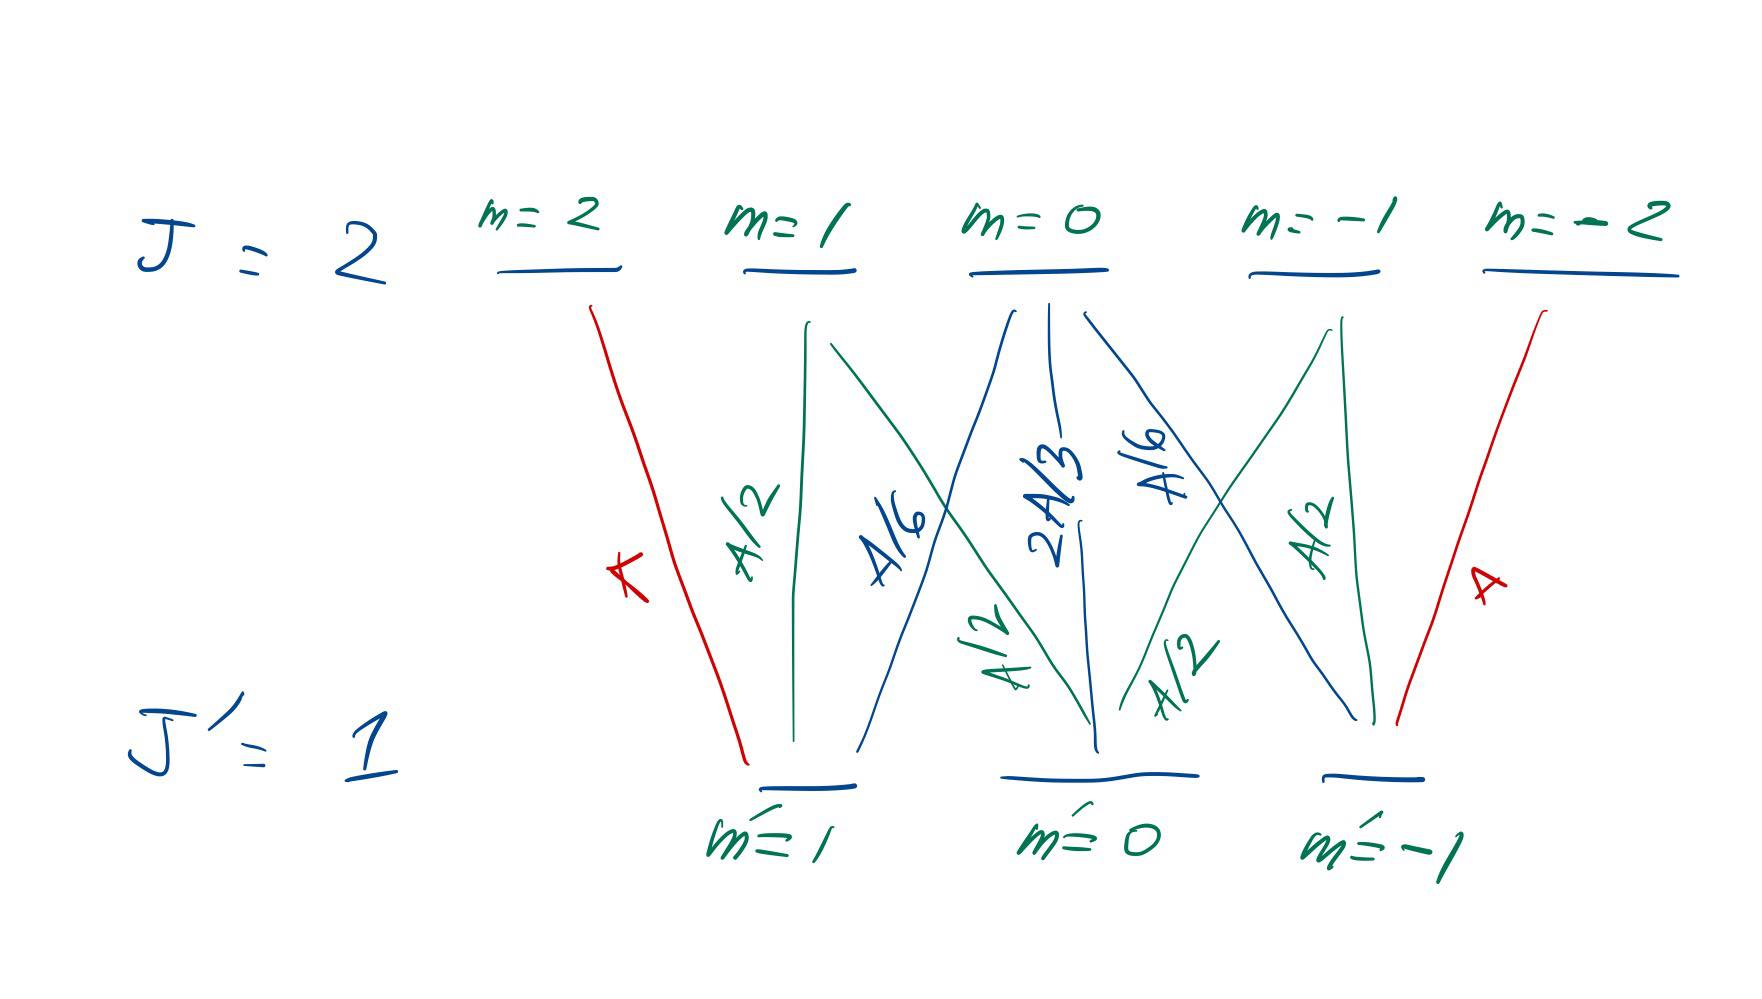
\includegraphics[width=0.9\textwidth]{branches.jpg}
		\caption{Transition rates.}
		\label{fig:1}
	\end{figure}
	$\,$\\
	$\,$\\
	$\,$\\
	$\,$\\
	$\,$\\
	$\,$\\
	$\,$\\
	$\,$\\
	$\,$\\
	$\,$\\
	$\,$\\
	$\,$\\
	$\,$\\
	$\,$
	
	
\end{enumerate}
	
	
\end{document}








